\section{Preliminary Results}\label{section:results}

\begin{figure}
 \centering
 % Switch this out so can see the uncertainties
 % 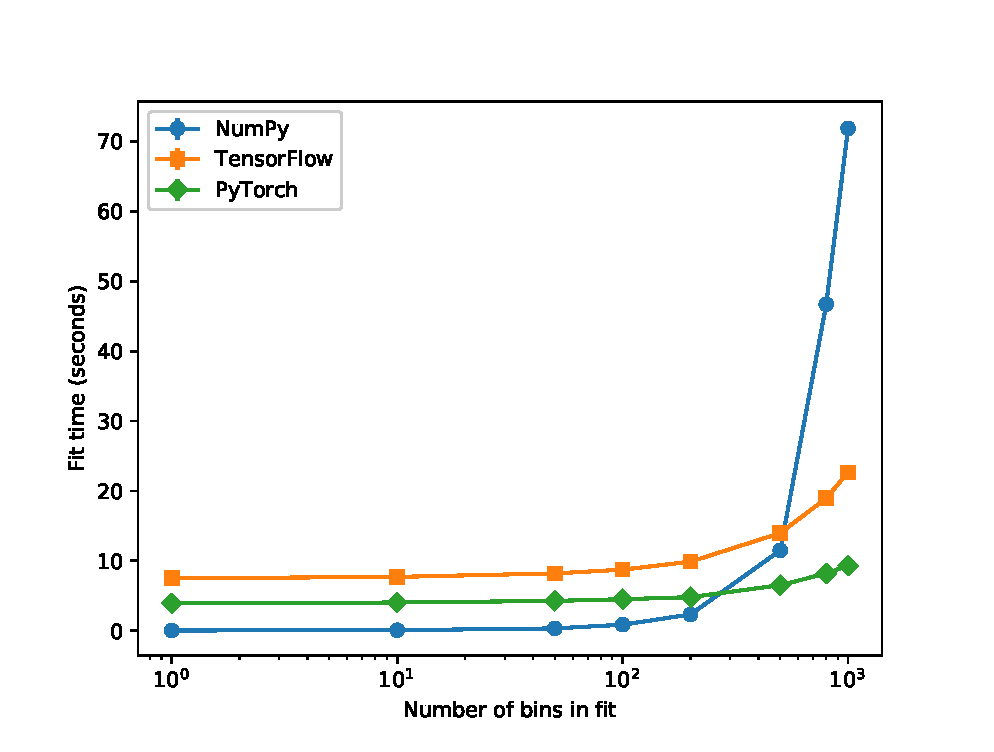
\includegraphics[width=0.9\linewidth]{benchmark_times.eps}
 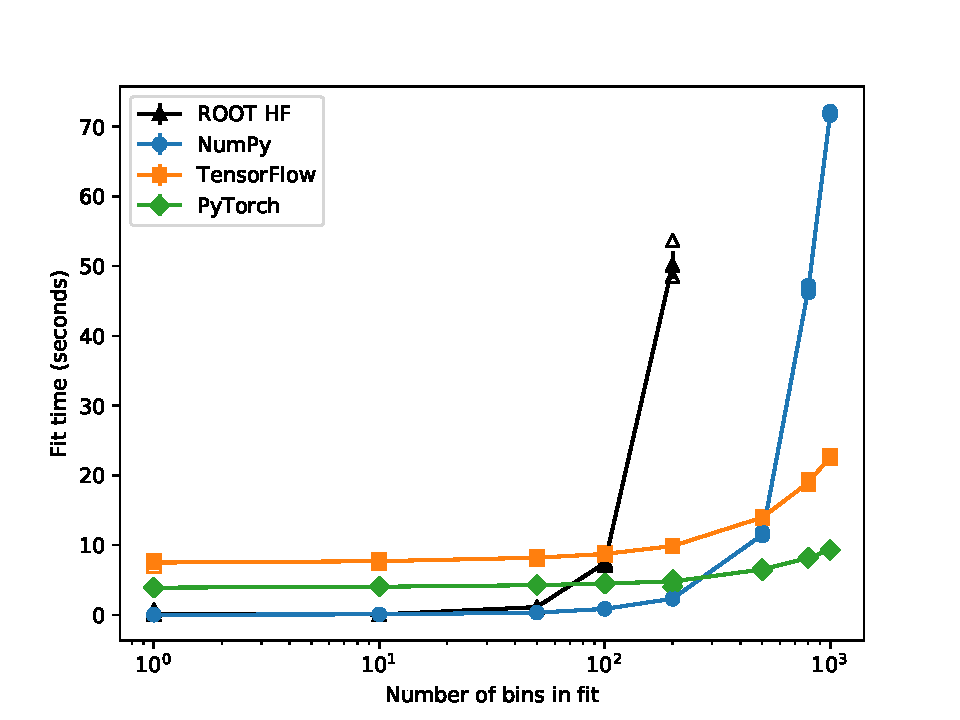
\includegraphics[width=0.9\linewidth]{benchmark_times.pdf}
 \caption{Comparison of the mean time needed to complete a one point CLs test for the NumPy, TensorFlow, and PyTorch pyhf backends vs. the number of bins in the associated fit.
  The model used is a simple one in which every bin has the same content to ensure that the fit will complete.
  In in lieu of model complexity large numbers of bins are given to simulate difficult conditions for the fit.
  The binning choices used are $n_{\text{bins}} \in \left\{1, 10, 50, 100, 200, 500, 800, 1000\right\}$.
  For each binning choice the fit is repeated 5 times.
  The minimum and maximum time for each run are shown as open shapes corresponding to the shapes of the markers for each backend, and an uncertainty bar corresponding to 1 standard deviation is drawn (though it may be obscured by the markers).
 }
 \label{fig:benchmark_backends}
\end{figure}

\begin{figure}
 \centering
 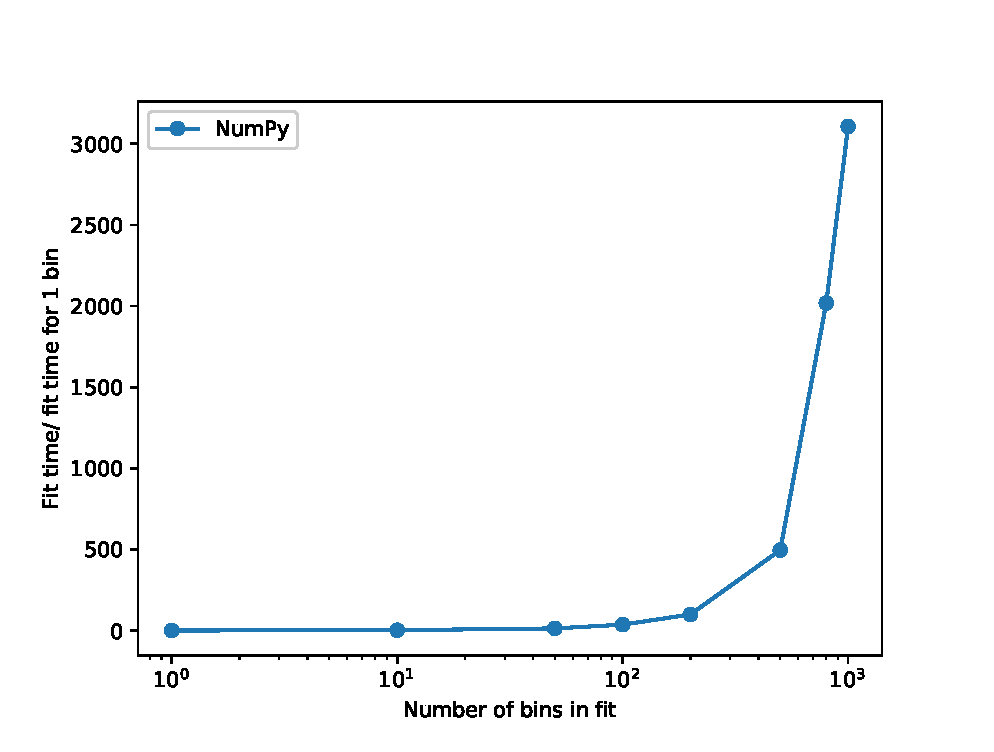
\includegraphics[width=0.6\linewidth]{relative_times_numpy_log.eps}
 \caption{Comparison of the mean time needed to complete a one point CLs test for the NumPy pyhf backend for a number of bins in the associated fit relative to the time for a single bin.
  The model used is a simple one in which every bin has the same content to ensure that the fit will complete.
  The binning choices used are $n_{\text{bins}} \in \left\{1, 10, 50, 100, 200, 500, 800, 1000\right\}$.
 }
 \label{fig:relative_time_numpy}
\end{figure}

\begin{figure}
 \centering
 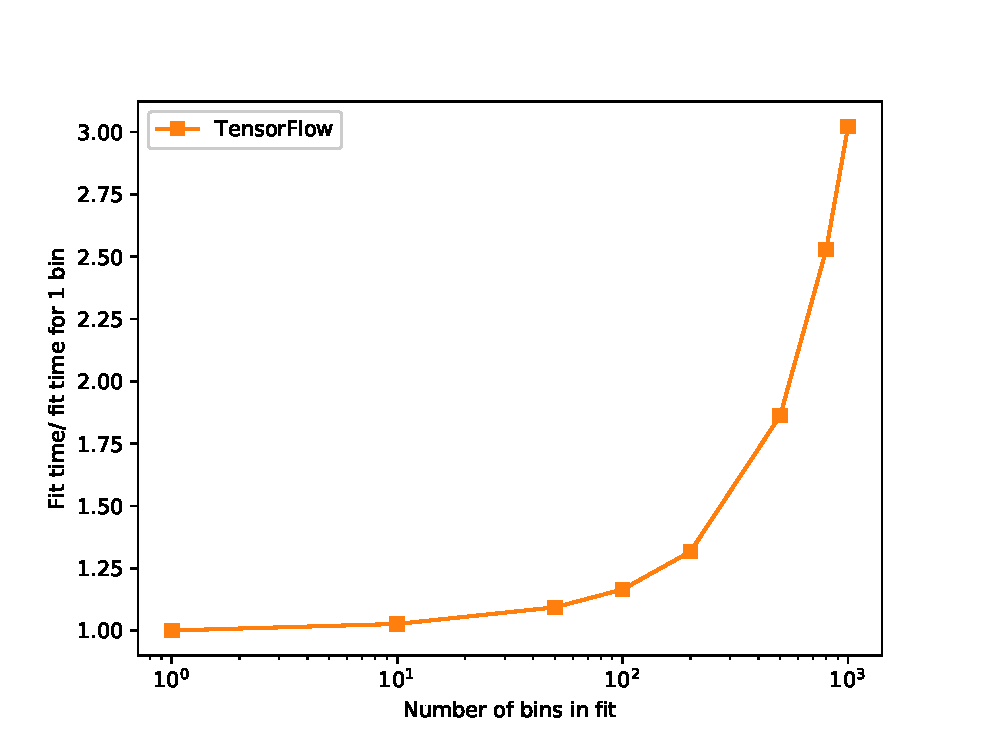
\includegraphics[width=0.6\linewidth]{relative_times_tensorflow_log.eps}
 \caption{Comparison of the mean time needed to complete a one point CLs test for the TensorFlow pyhf backend for a number of bins in the associated fit relative to the time for a single bin.
  The model used is a simple one in which every bin has the same content to ensure that the fit will complete.
  The binning choices used are $n_{\text{bins}} \in \left\{1, 10, 50, 100, 200, 500, 800, 1000\right\}$.
 }
 \label{fig:relative_time_tensorflow}
\end{figure}

\begin{figure}
 \centering
 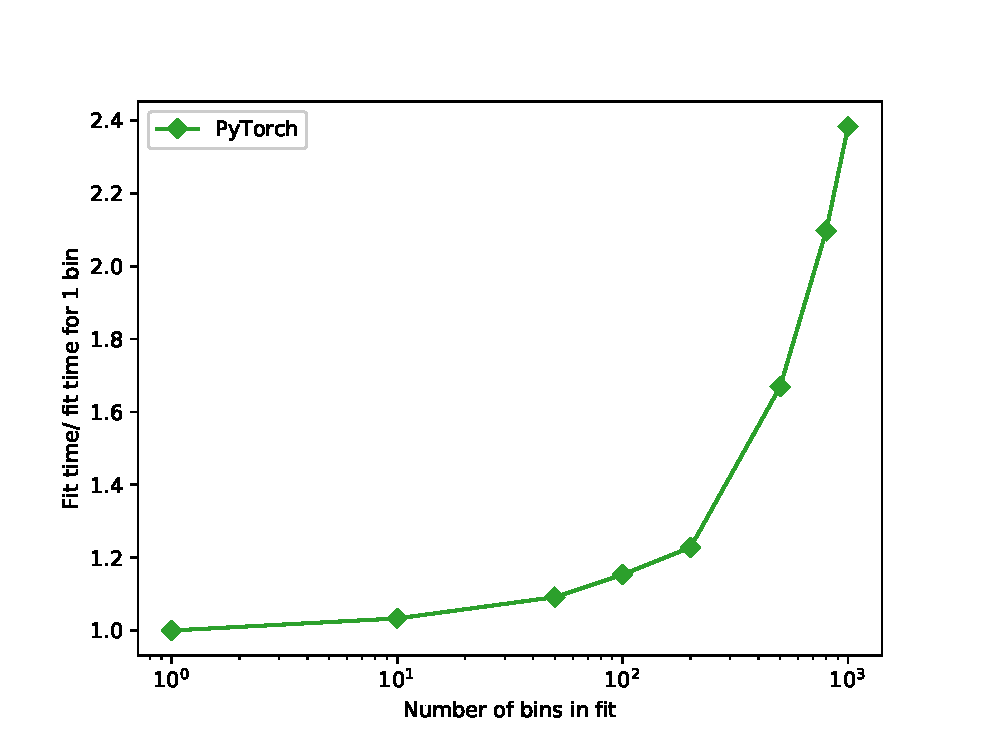
\includegraphics[width=0.6\linewidth]{relative_times_pytorch_log.eps}
 \caption{Comparison of the mean time needed to complete a one point CLs test for the PyTorch pyhf backend for a number of bins in the associated fit relative to the time for a single bin.
  The model used is a simple one in which every bin has the same content to ensure that the fit will complete.
  The binning choices used are $n_{\text{bins}} \in \left\{1, 10, 50, 100, 200, 500, 800, 1000\right\}$.
 }
 \label{fig:relative_time_pytorch}
\end{figure}
